
%(BEGIN_QUESTION)
% Copyright 2006, Tony R. Kuphaldt, released under the Creative Commons Attribution License (v 1.0)
% This means you may do almost anything with this work of mine, so long as you give me proper credit

One of the simplest linear operational amplifier circuit is the {\it voltage follower}, so-called because the output voltage very closely ``follows'' the input voltage within the opamp's operating range:

$$\includegraphics[width=15.5cm]{i01585x01.eps}$$

This approximation is so good that it is all but forgotten by most technicians, and most simply treat the circuit's behavior as $V_{out} = V_{in}$.  In actuality, though, there will always be a slight difference between the input and output voltages.  The difference is not difficult to calculate.  Suppose we have a perfect operational amplifier (zero noise, no offset voltage, no input bias current) with an internal (differential) voltage gain of 50,000:

$$\includegraphics[width=15.5cm]{i01585x02.eps}$$

Labeling the input and output terminal voltages (with reference to ground, of course) as the variables $a$, $b$, and $c$, we have a transfer function for the opamp that looks like this:

$$c = 50,000 (a - b)$$

If we connect the output of the opamp to its inverting input for negative feedback, we eliminate one of the variables from the equation because now the output terminal and the ($-$) input terminal are electrically common:

$$\includegraphics[width=15.5cm]{i01585x03.eps}$$

$$c = 50,000 (a - c)$$

Solve for the output voltage of this voltage follower circuit ($c$) when the input voltage ($a$) is exactly 5 volts, and explain why the output and input voltages are not precisely equal.  Then solve for the output voltage when the input voltage is exactly 5 volts and the opamp's gain is only 20,000 instead of 50,000.

\vskip 20pt \vbox{\hrule \hbox{\strut \vrule{} {\bf Suggestions for Socratic discussion} \vrule} \hrule}

\begin{itemize}
\item{} In general terms, would you say negative feedback {\it increases} or {\it decreases} the overall gain of an amplifier system?
\item{} What do you suppose would happen if we configured the operational amplifier for {\it positive} feedback instead of negative feedback?  How would it behave then?
\end{itemize}

\underbar{file i01585}
%(END_QUESTION)





%(BEGIN_ANSWER)

$$c = A_V (a - c)$$

$$c = A_V a - A_V c$$

$$c + A_V c = A_V a$$

$$c (1 + A_V) = A_V a$$

$$c = {A_V a \over {1 + A_V}}$$

$c$ = 4.999750012 volts when $a$ = 5.0000 volts (exactly) and $A_V$ = 20,000.  

\vskip 10pt

Increasing the intrinsic differential gain of the opamp will decrease the ``error'' between output and input.


%(END_ANSWER)





%(BEGIN_NOTES)


%INDEX% Electronics review: opamp voltage follower

%(END_NOTES)


